\subsection{Neo4j}

\par O Neo4j foi criado no início do século XXI por desenvolvedores que queriam resolver um problema em uma empresa de mídias. Porém, eles não obtiveram êxito ao tentar resolver tal problema utilizando as tecnologias tradicionais, portanto, decidiram arriscar e criar algo novo. A princípio, o Neo4j não era um sistema de gerenciamento de banco de dados orientado a grafos como é conhecido nos dias atuais. Ele era mais parecido com uma \textit{graph library} (biblioteca de grafo) em que as pessoas poderiam usar em seus projetos \cite{bruggen_learning_neo4j}.

\par De acordo com \citeonline{bruggen_learning_neo4j}, inicialmente ele foi desenvolvido para ser utilizado em conjunto com alguns bancos de dados relacionais como MySQL e outros, com a intenção de criar uma camada de abstração dos dados em grafos. Mas com o passar dos anos, os desenvolvedores decidiram tirar o Neo4j da estrutura dos bancos relacionais e criar sua própria estrutura de armazenamento em grafos.

\par O Neo4j, como vários outros, também é um projeto de sistema de gerenciamento de banco de dados NoSQL de código fonte aberto.

\par Segundo \citeonline{robinson_webber_eifrem_graph_databases}, os bancos de dados orientados a grafos possuem como diferencial a sua performance, agilidade e flexibilidade. Entretanto, a performance é o que mais se destaca entre eles, pois, a maneira como armazenam e realizam buscas no banco de dados é diferente dos bancos convencionais. Primeiramente, esse tipo de banco de dados não utiliza tabela; ele armazena os dados em vértices e arestas. Isso permite realizar buscas extremamente velozes através de \textit{traversals} (travessias), uma vez que estas implementam algoritmos para otimizar tais funcionalidades, evitando assim o uso de \textit{joins} complexos, tornando-o tão veloz.

\par \citeonline[p. 2]{neo4j_team_manual} afirma que:

\begin{citacao}
	\textit{A single server instance can handle a graph of billions of nodes and relationships. When data throughput is insufficient, the graph database can be distributed among multiple servers in a high availability configuration.}\footnotemark[11]
\end{citacao}

\footnotetext[11]{Um único servidor pode manipular um grafo de bilhões de nós e relacionamentos. Quando a taxa de transferência de dados é insuficiente, o banco de dados orientado a grafo pode ser distribuído entre vários servidores mantendo a mesma velocidade de processamento.}

\par Com estas informações, é possível mensurar o quanto o Neo4j pode ser rápido e robusto, sendo possível, até mesmo distribuí-lo a fim de obter uma melhor configuração, organização e facilidade de manutenção.

%BANCA_QUALIFICACAO. Comentado este parágrafo, porém o mesmo retornará para a banca de qualificação
\par Segundo \citeonline{neo4j_team_manual}, o banco de dados Neo4j é composto por nós (vértices), relacionamentos (arestas) e propriedades. Os relacionamentos são responsáveis por organizar os nós e ambos podem possuir seus atributos. É possível realizar as buscas e/ou alterações no Neo4j de duas formas diferentes. Sendo a primeira através da API \textit{Cypher Query Language}, que é uma \textit{query language} para banco de dados orientado a grafos muito próxima da linguagem humana, cuja descrição completa será apresentada a seguir. A segunda é o \textit{framework\footnotemark[12] Traversal} que utiliza a API \textit{Cypher} internamente para navegar pelo grafo.

\footnotetext[12]{\textit{Framework} - Abstração que une códigos comuns entre vários projetos de software, a fim de obter uma funcionalidade genérica.}


\citeonline{rocha_algoritmos_particionamento_banco_dados_orientado_grafos} afirma que o Neo4j permite criar mais de um relacionamento entre o mesmo par de vértices, desde que estes sejam de tipos distintos. Isso possibilita navegar pelos vértices do grafo de forma mais rápida devido a esses diferentes tipos de arestas, o que torna possível implementar o algoritmo de busca desejado. A Figura~\ref{fig:grafo_simples_neo4j} exemplifica um simples grafo utilizando um banco de dados Neo4j.

\begin{figure}[h!]
	\centerline{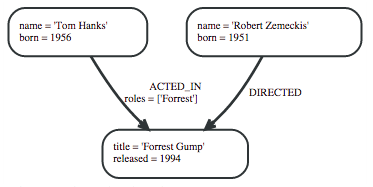
\includegraphics[scale=0.8]{./imagens/simple_graph_neo4j.png}}
	\caption[Exemplo simples de um grafo armazenado no Neo4j]
	{Exemplo simples de um grafo armazenado no Neo4j. \textbf{Fonte:} \citeonline{neo4j_team_manual}.}
	\label{fig:grafo_simples_neo4j}
\end{figure}

%BANCA_QUALIFICACAO. Comentado este parágrafo, porém o mesmo retornará para a banca de qualificação
\par Há duas formas de executar o Neo4j, segundo \citeonline{robinson_webber_eifrem_graph_databases}. A primeira é conhecida como \textit{Server} e a segunda \textit{Embedded}. O modo \textit{Server} é utilizado principalmente em \textit{web-service} em conjunto com a API REST, este será aplicado neste trabalho. Já no modo \textit{Embedded} o banco de dados é executado embarcado à aplicação Java.

%BANCA_QUALIFICACAO. Comentado este parágrafo, porém o mesmo retornará para a banca de qualificação
\par Conforme \citeonline{neo4j_team_manual}, o Neo4j possui suporte as transações ACID (com atomicidade, consistência, isolamento e durabilidade).

O Neo4j é distribuído em duas versões sendo elas a \textit{Entreprise} e a \textit{Community}. A primeira possui um tempo de avaliação de 30 dias e após esse tempo, é necessário comprar uma licença para continuar a utilizá-lo. Como diferencial essa versão possui ferramentas para o gerenciamento do banco de dados, incluindo melhorias relacionadas à escalabilidade. A segunda versão é disponibilizada gratuitamente sem data limite de expiração, contudo, ela não possui os recursos mencionados anteriormente que estão presentes na versão \textit{Enterprise}, mas é muito utilizada para fins didáticos e para pequenos projetos, aplicando-se perfeitamente a este projeto \cite{neo4j_team_manual}.

\par Por ser um banco de dados orientado a grafo bastante robusto, seguro e possuir uma documentação de fácil entendimento, além, é claro, de possuir um baixo custo de implantação devido a sua licença \textit{open source}, esse banco de dados foi escolhido para ser utilizado neste trabalho.
